% ============================================================================
% An Adaptive Knowledge-Based System for PPh 21 Calculation with LLM-Assisted
% Knowledge Acquisition from Regulations and Company Policies
%
% English version of paper.tex (Indonesian). Keep the two files in step.
% Format  : IEEE conference template (IEEEtran, conference option), 8-page target
% Build   : pdflatex, bibtex, then pdflatex twice (in paper/draft/)
% Numbers : same as paper.tex and paper_lengkap.tex.
% Figures : gambar_replay_en.tex is generated by system/tools/paper_figures.py
%           from the experiment logs.
% ============================================================================
\documentclass[conference]{IEEEtran}
% The next template line is only for funding in the first footnote; there is none.
%\IEEEoverridecommandlockouts
\usepackage{cite}
\usepackage{amsmath,amssymb,amsfonts}
\usepackage{algorithmic}
\usepackage{graphicx}
\usepackage{textcomp}
\usepackage{xcolor}
\def\BibTeX{{\rm B\kern-.05em{\sc i\kern-.025em b}\kern-.08em
    T\kern-.1667em\lower.7ex\hbox{E}\kern-.125emX}}

% Additions to the template. None of them changes margins, columns, or fonts.
\usepackage[T1]{fontenc}
\usepackage{amsthm,mathtools}
\usepackage{booktabs}
\usepackage{tabularx}
\usepackage{array}
\usepackage{tikz}
\usetikzlibrary{positioning,arrows.meta,fit,calc}
\usepackage{pgfplots}
\pgfplotsset{compat=1.16}
\usepackage{url}
% Reference entries use \nolinkurl from hyperref, which the template does not load.
\providecommand{\nolinkurl}[1]{\url{#1}}

\newcolumntype{L}{>{\raggedright\arraybackslash}X}
\newcolumntype{P}[1]{>{\raggedright\arraybackslash}p{#1}}

\newtheorem{definition}{Definition}

% Notation: x = test case, t = tax period, \omega = knowledge date,
% m = number of candidates, n = event index.
\newcommand{\K}{\mathcal{K}}
\newcommand{\result}{\mathit{result}}
\newcommand{\gold}{\star}
\newcommand{\SG}{S^{G}}
\newcommand{\SE}{S^{E}}

\tikzset{
  flowbox/.style={draw, rounded corners=2pt, align=center, font=\footnotesize, inner sep=2pt, minimum height=0.6cm},
  databox/.style={draw, align=center, font=\footnotesize, inner sep=2pt, minimum height=0.6cm, fill=gray!10},
  arrow/.style={-{Stealth[length=2mm]}, semithick}
}

\begin{document}
% Six or more authors are written "et al." as the template asks; the control entry is in rujukan_tambahan.bib
\bstctlcite{IEEEexample:BSTcontrol}

\title{An Adaptive Knowledge-Based System for PPh 21 Calculation with LLM-Assisted Knowledge Acquisition from Regulations and Company Policies}

\author{\IEEEauthorblockN{1\textsuperscript{st} Obi Kastanya}
\IEEEauthorblockA{\textit{Department of Informatics} \\
\textit{Institut Teknologi Sepuluh Nopember}\\
Surabaya, Indonesia \\
6025252015@student.its.ac.id}
\and
\IEEEauthorblockN{2\textsuperscript{nd} Mahathir Muhammad}
\IEEEauthorblockA{\textit{Department of Informatics} \\
\textit{Institut Teknologi Sepuluh Nopember}\\
Surabaya, Indonesia \\
6025252008@student.its.ac.id}
}

\maketitle

\begin{abstract}
Indonesian Income Tax Article 21 calculation must follow changes in regulations and company policies, but its rules are embedded in code. Tax formalization with large language models (LLMs) usually builds a rule base from scratch for a single legal state, so it is unknown whether repeated updates preserve past-period results and whether errors propagate. This study proposes a knowledge-based system with a two-layer bitemporal knowledge base and incremental LLM-assisted acquisition, checked by five verification gates and behavioral consensus, that abstains when uncertain. The evaluation replays 13 real regulatory changes from 2023 to 2026 with 20 distractors and tests 16 unseen changes. The core design was locked before the experiments, while ablations, a second model, and the regeneration chain were added after early results were visible. Gold reference data and test changes were reviewed only by AI agents, not human experts. The representation expresses 16 of 16 changes without modifying the engine (one-sided 95 percent lower bound 0.829), provided that the rounding convention of the examples is aligned. On 18 real documents, undetected wrong updates occurred on 3 (upper bound 0.377, above the 0.25 threshold) and correct updates on 8 (confidence interval 0.215 to 0.692), no higher than the baselines. In chained mode, 31 of 33 events added no new errors (lower bound 0.821), but only 23 of 33 on the regenerated chain (lower bound 0.540). Recall of cross-layer impact detection was 0.91 (confidence interval 0.75 to 1.00). LLMs can draft updates, but a human reviewer remains necessary.
\end{abstract}

\begin{IEEEkeywords}
knowledge acquisition, knowledge-based system, knowledge graph, large language model, PPh Article 21, regulatory change, rules as code
\end{IEEEkeywords}

% ============================================================================
\section{Introduction}
\label{sec:pendahuluan}
% ============================================================================
Income Tax (PPh) Article 21 is withheld every month from the income of Indonesian employees, so a calculation error directly affects every payslip. Its regulations change often. Our corpus records 13 events that changed the PPh 21 calculation for permanent employees in 2023--2026, seven of them issued in 2025. They vary in type: Pension Security wage caps, the classification of benefits in kind, the government-borne tax (DTP) facility, rounding rules, and in 2024 a change of method to the average effective rate (TER)~\cite{pp58_2023,pmk168_2023}.

In current practice, tax rules are embedded in code or spreadsheets~\cite{ramadhani2021grossup,kusuma2026pph21}. Every change requires reprogramming. As an illustration from two open-source repositories, one added TER 26 days after Government Regulation (PP) 58/2023 was issued and the other 915 days after. There is no evidence that such changes leave past-period results intact, and company policies that become noncompliant go undetected.

Knowledge-based systems (KBSs) separate knowledge from code~\cite{merigoux2021catala}, but they shift the burden to maintaining the knowledge base (KB). Large language models (LLMs) can translate legal text into rules~\cite{janatian2023texttostructure}, but they are unreliable for calculations that demand exactness~\cite{nay2024taxattorneys,dahl2024legalfictions}. LLM-assisted tax formalization usually builds a rule base from scratch for the law at one point in time. To the best of our knowledge as of November 2026, no study has measured three things on an executed legal rule base: whether repeated LLM updates preserve past-period results, whether errors propagate from one change to the next, and how the updates affect a company policy layer.

We propose a KBS whose knowledge is stored as a two-layer bitemporal knowledge graph and run by a deterministic inference engine (Fig.~\ref{fig:alur}). The LLM does not compute tax. It only drafts candidate updates $\Delta$, five verification gates filter them, behavioral consensus selects one, and the system abstains when no candidate is convincing.

\begin{figure}[t]
\centering
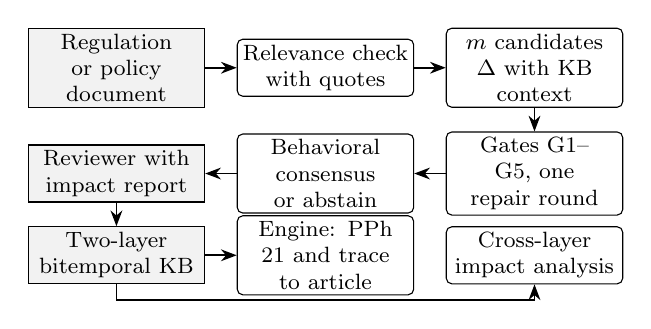
\begin{tikzpicture}[node distance=3mm and 4mm]
\node[databox, text width=2.1cm] (dok) {Regulation or policy document};
\node[flowbox, right=of dok, text width=2.1cm] (rel) {Relevance check with quotes};
\node[flowbox, right=of rel, text width=2.1cm] (m) {$m$ candidates $\Delta$ with KB context};
\node[flowbox, below=of m, text width=2.1cm] (g) {Gates G1--G5, one repair round};
\node[flowbox, left=of g, text width=2.1cm] (k) {Behavioral consensus or abstain};
\node[databox, left=of k, text width=2.1cm] (rev) {Reviewer with impact report};
\node[databox, below=of rev, text width=2.1cm] (kb) {Two-layer bitemporal KB};
\node[flowbox, right=of kb, text width=2.1cm] (eng) {Engine: PPh 21 and trace to article};
\node[flowbox, right=of eng, text width=2.1cm] (d) {Cross-layer impact analysis};
\draw[arrow] (dok) -- (rel);
\draw[arrow] (rel) -- (m);
\draw[arrow] (m) -- (g);
\draw[arrow] (g) -- (k);
\draw[arrow] (k) -- (rev);
\draw[arrow] (rev) -- (kb);
\draw[arrow] (kb) -- (eng);
\draw[arrow] (kb.south) -- ++(0,-2mm) -| (d.south);
\end{tikzpicture}
\caption{System overview and acquisition flow. The LLM only drafts candidates. A deterministic engine computes over the KB.}
\label{fig:alur}
\end{figure}

We answer four research questions (RQs). RQ1 asks to what extent the representation can express regulatory and policy changes, including changes unknown at design time, without modifying engine code. RQ2 asks how often LLM-assisted acquisition applies correct and wrong updates, and what role the gates play. RQ3 asks how many real events are applied automatically and whether errors propagate. RQ4 asks how completely the system finds affected company policies.

Our contributions are (1) a two-layer temporal representation with conflict resolution and cross-layer impact analysis, (2) an incremental acquisition method with verification gates, a nonvacuity gate, and behavioral consensus, (3) definitions of representational and operational adaptivity and a regulation replay protocol that separates inherited, new, and triggered errors, and (4) artifacts comprising the KB, corpus, gold updates, test suite, and evaluation code.

% ============================================================================
\section{Background}
\label{sec:masalah}
% ============================================================================
PPh 21 for permanent employees is computed from gross income less occupational expenses, contributions, and the nontaxable income amount, and annual taxable income (PKP) is then taxed at the progressive rates of Article 17 in five brackets of 5\%--35\%~\cite{uu7_2021,pmk101_2016}. Until 2023, the tax of each period was computed by annualizing income~\cite{per16_2016}. Since 2024, January to November use a monthly TER with 125 brackets in categories A, B, and C, and the last period recomputes the full year~\cite{pp58_2023,pmk168_2023}. The DTP facility of 2025--2026 adds sector criteria and income caps~\cite{pmk10_2025,pmk105_2025}.

Companies decide components such as proration, the religious holiday allowance, and who bears the tax, but they may not deviate from mandatory provisions. For example, Article 22(3) of the 2025--2026 collective labor agreement (PKB) of PT Wijaya Karya states that government tax incentives are not given to employees, whereas Article 5(1) of Minister of Finance Regulation (PMK) 10/2025 requires DTP to be paid in cash~\cite{pmk10_2025}. This conflict is latent because the company is not in a DTP sector. Taxonomies of change types (T1--T10) and conflict types (C1--C10) were fixed before any LLM output existed. The scope is permanent employees of private or state-owned employers.

% ============================================================================
\section{Related Work}
\label{sec:terkait}
% ============================================================================
Rules-as-code systems such as Catala~\cite{merigoux2021catala} and DataLex~\cite{mowbray2023scaling} formalize legislation as programs, but humans write the knowledge. Ripple-Down Rules add rules incrementally with cornerstone cases as a regression guard~\cite{compton2021rdr}, which is equivalent to our gate G4, but an expert still writes each change.

The closest group uses LLMs. Veeramani et al.\ store the Indian Income Tax Act as a knowledge graph and reach 80\% accuracy on 20 scenarios~\cite{veeramani2026neurosymbolic}. Yadamsuren et al.\ formalize one section of the United States (US) Internal Revenue Code in Prolog~\cite{yadamsuren2026formalization}. Lorenzo et al.\ translate French tax provisions into Catala without executing the output~\cite{lorenzo2025translating}. Jurayj et al.\ combine LLMs with a Prolog solver on 100 cases, where o3 gives 75 correct, 15 wrong, and 10 abstained~\cite{jurayj2026tax}. These works formalize one legal state. The nearest exception is Gogani-Khiabani et al., who ask an LLM to update US tax code from 2020 to 2021 and select candidates by behavioral majority vote~\cite{goganikhiabani2025maintaining}, but only for one step and without testing past periods.

Sequential editing of LLM knowledge damages model abilities~\cite{gupta2024editing}, although KoLEG keeps performance above 95\% after four edits from Korean legal amendments~\cite{seo2025koleg}. There the model is edited, not a rule base. Prior et al.\ consolidate German statutes with an LLM, and exact match falls from 50.3\% for one step to 20.51\% for amendment chains~\cite{prior2025risks}, but the object is text, not executed rules. The metrics of RQ2 and RQ3 build on pass@k~\cite{chen2021evaluating}, n@k~\cite{li2022alphacode}, and selective prediction~\cite{xin2021abstention}. Table~\ref{tab:posisi} summarizes our position.

\begin{table}[t]
\centering
\caption{Position Relative to the Closest Work (Incr. = Incremental Update, Prop. = Error Propagation Measured, Co. = Company Layer)}
\label{tab:posisi}
\scriptsize
\setlength{\tabcolsep}{3pt}
\begin{tabularx}{\columnwidth}{@{}P{2.15cm} L P{1.1cm} P{0.85cm} P{0.9cm} P{0.45cm}@{}}
\toprule
\textbf{Work} & \textbf{Representation} & \textbf{Author} & \textbf{Incr.} & \textbf{Prop.} & \textbf{Co.} \\
\midrule
Catala~\cite{merigoux2021catala} & domain-specific language & human & -- & -- & -- \\
Ripple-Down Rules~\cite{compton2021rdr} & rules, exceptions & expert & yes & -- & -- \\
Veeramani et al.~\cite{veeramani2026neurosymbolic} & graph, symbolic rules & LLM, expert & idea & -- & -- \\
Yadamsuren et al.~\cite{yadamsuren2026formalization} & Prolog & LLM & -- & -- & -- \\
Lorenzo et al.~\cite{lorenzo2025translating} & Catala & LLM & -- & -- & -- \\
Jurayj et al.~\cite{jurayj2026tax} & Prolog & LLM & -- & -- & -- \\
Gogani-Khiabani et al.~\cite{goganikhiabani2025maintaining} & Python code & LLM & one step & -- & -- \\
Prior et al.~\cite{prior2025risks} & XML text & LLM & text & partial & -- \\
\midrule
\textbf{This study} & bitemporal graph and executed rules & LLM, gates & yes & yes & yes \\
\bottomrule
\end{tabularx}
\end{table}

% ============================================================================
\section{Representation and Inference Engine}
\label{sec:representasi}
% ============================================================================
Structural knowledge, namely documents, articles, rules, parameters, tables, policies, versions, and their relations, is stored as a Resource Description Framework (RDF) and Web Ontology Language (OWL) knowledge graph in GraphDB, validated with the Shapes Constraint Language (SHACL)~\cite{knublauch2017shacl} and queried with SPARQL. The ontology reuses the European Legislation Identifier (ELI)~\cite{publicationsoffice2026elien}, OWL-Time~\cite{cox2017owltime}, and PROV-O~\cite{lebo2013provo}. Calculation expressions are stored as rule attributes and run by the engine, because tax arithmetic demands rupiah exactness, exact fractions, and fixed-point iteration. With this split, a regulatory change touches only graph data. Fig.~\ref{fig:ontologi} shows the ontology.

\begin{figure*}[t]
\centering
\newcommand{\ontologicatatan}{Every pph:KBElement: elementId, seq, recordedOn ($\approx$ prov:generatedAtTime), validFrom, validUntil ($\approx$ time:ProperInterval);\\
   one named graph kb:update/\textit{id} per update. pph:Rule: layer $\in$ \{Regulation, Company\}, modality $\in$ \{Mandatory, Default, Optional\},\\
   scope $\in$ \{Period, Year\}, expression, condition, fixed point, policy.}
% Ontologi knowledge graph (docs/gambar/ontologi.tex) dengan label 8 pt Times sesuai templat IEEE.
% Keterangan di bawah gambar dapat diganti lewat \ontologicatatan (paper_en.tex memakainya).
\providecommand{\ontologicatatan}{Setiap pph:KBElement: elementId, seq, recordedOn ($\approx$ prov:generatedAtTime), validFrom, validUntil\\
   ($\approx$ time:ProperInterval); satu \en{named graph} kb:update/\textit{id} per pembaruan. pph:Rule: layer $\in$ \{Regulation, Company\},\\
   modality $\in$ \{Mandatory, Default, Optional\}, scope $\in$ \{Period, Year\}, expression, condition, fixed point, policy.}
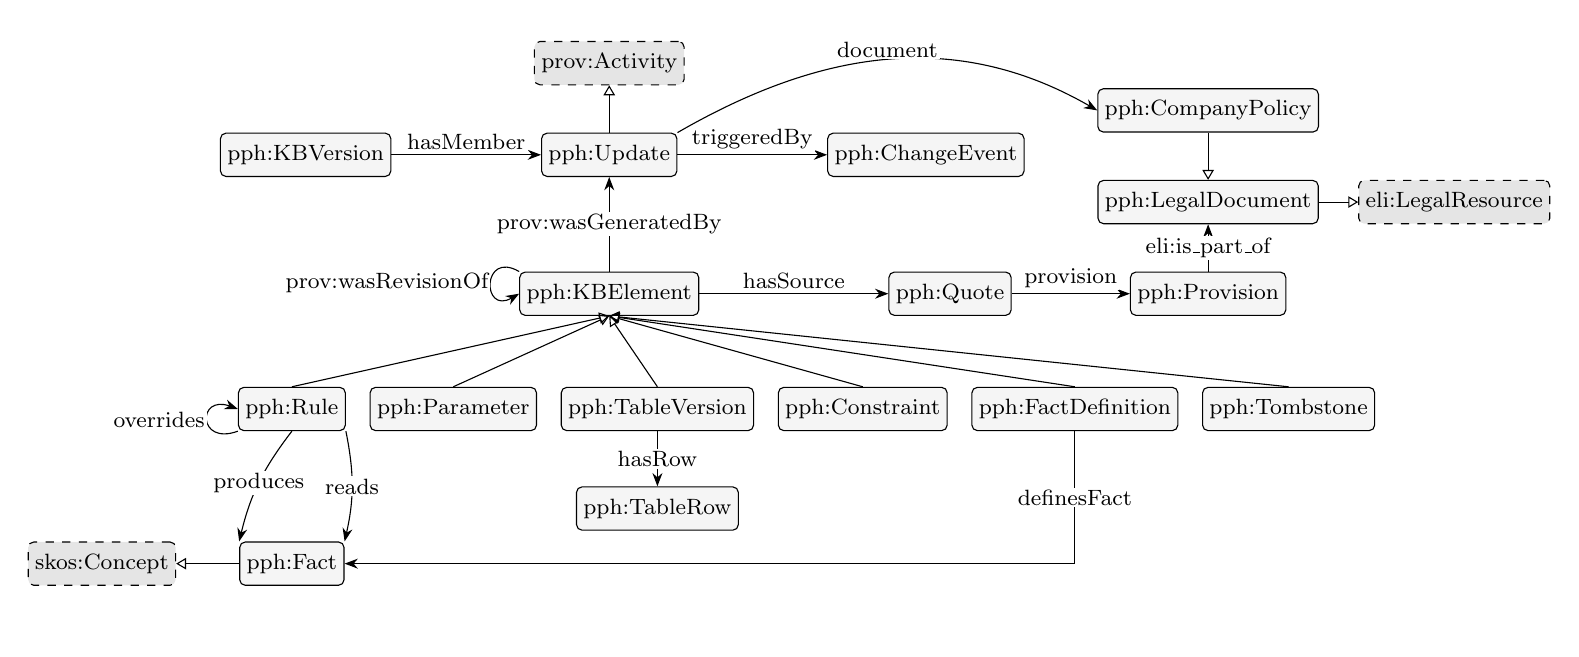
\begin{tikzpicture}[
  node distance=6mm and 7mm,
  cls/.style={draw,rounded corners=2pt,fill=gray!8,font=\footnotesize,minimum height=5.5mm,inner sep=2.5pt},
  ext/.style={cls,fill=gray!20,dashed},
  sub/.style={-{Triangle[open]},thin},
  rel/.style={-{Stealth},thin},
  lab/.style={font=\footnotesize,fill=white,inner sep=0.8pt}]

% unsur knowledge base
\node[cls] (el) {pph:KBElement};
\node[cls,below left=9mm and 22mm of el] (rule) {pph:Rule};
\node[cls,right=3mm of rule] (par) {pph:Parameter};
\node[cls,right=3mm of par] (tab) {pph:TableVersion};
\node[cls,right=3mm of tab] (con) {pph:Constraint};
\node[cls,right=3mm of con] (fd) {pph:FactDefinition};
\node[cls,right=3mm of fd] (tomb) {pph:Tombstone};
\foreach \n in {rule,par,tab,con,fd,tomb} \draw[sub] (\n.north) -- (el.south);
\node[cls,below=7mm of tab] (row) {pph:TableRow};
\draw[rel] (tab) -- node[lab]{hasRow} (row);

% fakta
\node[cls,below=14mm of rule] (fact) {pph:Fact};
\node[ext,left=8mm of fact] (concept) {skos:Concept};
\draw[sub] (fact) -- (concept);
\draw[rel] (rule.south) to[bend right=12] node[lab]{produces} (fact.north west);
\draw[rel] (rule.south east) to[bend left=12] node[lab]{reads} (fact.north east);
\draw[rel] (fd.south) |- node[lab,pos=0.25]{definesFact} (fact.east);
\draw[rel] (rule.south west) to[out=200,in=160,looseness=5] node[lab,left]{overrides} (rule.west);

% asal-usul
\node[cls,right=24mm of el] (quote) {pph:Quote};
\node[cls,right=15mm of quote] (prov) {pph:Provision};
\node[cls,above=6mm of prov] (doc) {pph:LegalDocument};
\node[ext,right=5mm of doc] (eli) {eli:LegalResource};
\node[cls,above=6mm of doc] (pol) {pph:CompanyPolicy};
\draw[rel] (el) -- node[lab,above=1pt]{hasSource} (quote);
\draw[rel] (quote) -- node[lab,above=1pt]{provision} (prov);
\draw[rel] (prov) -- node[lab]{eli:is\_part\_of} (doc);
\draw[sub] (doc) -- (eli);
\draw[sub] (pol) -- (doc);

% perubahan dan versi
\node[cls,above=12mm of el] (upd) {pph:Update};
\node[cls,left=19mm of upd] (ver) {pph:KBVersion};
\node[cls,right=19mm of upd] (ev) {pph:ChangeEvent};
\node[ext,above=6mm of upd] (act) {prov:Activity};
\draw[rel] (el) -- node[lab]{prov:wasGeneratedBy} (upd);
\draw[rel] (ver) -- node[lab,above=1pt]{hasMember} (upd);
\draw[rel] (upd) -- node[lab,above=1pt]{triggeredBy} (ev);
\draw[sub] (upd) -- (act);
\draw[rel] (upd.north east) to[out=30,in=150] node[lab,above]{document} (pol.west);
\draw[rel] (el.north west) to[out=150,in=210,looseness=5] node[lab,left]{prov:wasRevisionOf} (el.west);

\node[font=\footnotesize,align=left,anchor=north west] at ([yshift=-3mm]concept.south west)
  {\ontologicatatan};
\end{tikzpicture}

\caption{Knowledge base ontology. The main classes are legal document, article, quote, KB element, fact concept, company policy, change event, update, and KB version.}
\label{fig:ontologi}
\end{figure*}

\begin{definition}[Knowledge Base]
\label{def:kb}
$\K$ holds rule records, versioned parameters, table versions, mandatory constraints, and source documents. A rule $r = \langle \mathit{id}, \ell, \sigma, [t_s, t_e], t_c, \varphi, f \coloneqq e, \mathit{ov}, \mathit{src} \rangle$ has a layer $\ell$ (regulation or company), a nature $\sigma$ (mandatory, default, optional), a validity period, a recording date $t_c$ (the publication date of the document), a condition, a fact with its expression, the rules it overrides, and a source quote. Records are never edited in place.
\end{definition}

\begin{definition}[Calculation Result]
\label{def:hasil}
$\result(\K, x, t, \omega)$ is the value of an output fact for case $x$ in tax period $t$, computed with the regulations known on date $\omega$ plus the policy of the case. A case is one employee at one employer for one tax year, and the main fact is the PPh 21 due per period.
\end{definition}

The validity period $[t_s, t_e]$ and the knowledge time $t_c$ make $\K$ bitemporal, because a query at $\omega$ sees only records with $t_c \leq \omega$. For retroactive regulations, a query with $\omega \geq t_c$ gives the value that should have applied. When several rules are active for the same fact, the engine applies lex superior (mandatory regulation, company rule, adopted optional regulation, then default), lex specialis through an explicit \texttt{overrides} relation, and lex posterior. A company rule that loses to a mandatory rule with a different value is recorded as a conflict. The engine computes one case for a full year with demand-driven evaluation and fixed-point iteration for gross-up, and it records the trace of each fact down to the article. Expressions are limited to 27 registered functions and all arithmetic is exact, so a rounding change is a data update.

% ============================================================================
\section{LLM-Assisted Knowledge Acquisition}
\label{sec:akuisisi}
% ============================================================================
An update $\Delta$ for an event with publication date $t_{\mathit{pub}}$ and effective date $t_{\mathit{eff}}$ adds, changes, or removes elements, with $\K' = \K \oplus \Delta$. Gold updates satisfy $\K^{\gold}_n = \K^{\gold}_{n-1} \oplus \Delta^{\gold}_n$, and an empty $\Delta$ is the correct answer for a distractor.

\begin{definition}[Adaptive Conditions]
\label{def:syarat}
For a case set $S$: (A1) the engine code does not change; (A2) $\result(\K', x, t, \omega) = \result(\K^{\gold}, x, t, \omega)$ for $x \in S$, $t \geq t_{\mathit{eff}}$, and $\omega \geq t_{\mathit{pub}}$; (A3$_t$) results for $t < t_{\mathit{eff}}$ do not change; (A3$_\omega$) results for $\omega < t_{\mathit{pub}}$ do not change; (A4) the conflict report equals that of $\K^{\gold}$.
\end{definition}

\begin{definition}[Adaptivity]
\label{def:adapt}
A representation is adaptive to an event if there \emph{exists} a $\Delta$ that satisfies A1--A4 (RQ1). A system is operationally adaptive if the $\hat{\Delta}$ \emph{selected by the pipeline} satisfies A2, A3$_t$, and A4 on all of $\SE$, so one wrong observation makes $\hat{\Delta}$ wrong (RQ2, RQ3).
\end{definition}

A1 and A3$_\omega$ hold by construction and are checked as invariants, while A2, A3$_t$, and A4 are tested.

\textbf{Pipeline.} The document text is locked with SHA-256 and split by article. The LLM assesses relevance with quotes, then drafts $m$ independent candidates with KB context from SPARQL and a quote per element. Candidates that pass the gates, with one repair round, are grouped by output fact values and conflict reports on the gate cases $\SG$. The largest group wins, and a tie or the absence of a passing candidate means abstention. In operation, a reviewer checks the update before it takes effect.

\textbf{Gates.} G1 checks the schema, strict application, and 15 shapes and 12 SHACL-SPARQL constraints. G2 requires that quotes appear in the source text, that every new number and date appears in the quote of its element, and that $t_c = t_{\mathit{pub}}$. G3 checks expressions, the dependency graph, and references. G4 is a regression test on $\SG$, so results before the effect date and results with $\omega < t_{\mathit{pub}}$ must not change. G5 requires nonvacuity, so every added or changed element must change at least one output fact or conflict report on $\SG$, and a removed element must have fired. Without G5, an empty update passes all gates. $\SG$ is generated per candidate without reading gold data or $\SE$, holds at most 300 cases, and does not overlap $\SE$.

\textbf{Impact analysis.} A policy $P$ is \emph{affected} if the value of a fact of its rules changes, the winning rule of a fact that $P$ reads or produces changes, or a new conflict appears. These labels come from execution, whereas the detector is static. It computes $F_\Delta$, the facts touched by $\Delta$ with their downstream closure, and flags rules of $P$ that read those facts or produce the same fact as a rule in $\Delta$. Its query was frozen before E4.

\textbf{Configuration.} The main model is Claude Opus 5.5, and the second model is \texttt{gpt-6.1-sol}. Experiment calls ran on October 28--29, 2026, and were fully logged, so the analysis can be repeated without an LLM. Spending was about USD 81.6 for Claude and USD 8.1 for OpenAI.

% ============================================================================
\section{Evaluation Methodology}
\label{sec:evaluasi}
% ============================================================================
\textbf{Metrics.} RQ1 uses representational adaptability (RA), the proportion of unseen changes whose $\Delta$ reproduces all examples without modifying the engine. RQ2 uses the silent error rate (SER) and the correct application rate (CAR) over 13 regulations and 5 real PKBs, one result per document. RQ3 uses the operational adaptability rate (OAR), the proportion of events that add no new errors, and the triggered errors $I_n$, which are cases that are wrong in chained mode, are not wrong in isolated mode, and were not wrong before. RQ4 uses recall and $F_2$ over policy-event pairs. Table~\ref{tab:putusan} lists the hypotheses and thresholds.

\textbf{Design and preregistration.} This study follows design science research. Hypotheses, thresholds, data splits, the main test cases, the analysis plan, the acquisition pipeline, and the engine were locked at commit \texttt{c5983ff} (tags \texttt{prareg}, \texttt{alur-beku}, \texttt{engine-v1}) before the first test event ran. The gold data were also fixed at that commit. This lock uses git, which is weaker than third-party registration. Mutation analysis and 17 targeted cases entered at \texttt{d9c2886}, 42 minutes after the first E2 call, although the preregistration asked for them before E2. Both derive from gold data only and entered before E2 was scored. The initial budget of USD 15 ran out after the main E2 and E3 strata, so Amendment 1 (\texttt{2df0727}) was written after early results were visible, without changing the pipeline, engine, gold data, $\SE$, or thresholds. Apart from the nine remaining distractors, the second isolated run, and the regeneration chain, all amendment runs are exploratory.

\textbf{Data.} Development used 13 events from 2012--2022, five fictional regulations, and one PKB. Test data comprise 13 real events (E01--E13), 20 distractors whose correct answer is an empty update, five real PKBs, 14 synthetic policies, four counterfactual documents, and 16 unseen changes (U01--U16). Table~\ref{tab:korpus} details the test events. As of November 3, 2026, our search found no prospective event.

\begin{table}[t]
\centering
\caption{Test Corpus and E2 Results of the Proposed Method (C Correct, W Wrong, A Abstain). Rows SP and CF Ran Under Amendment 1; 2 of the 5 C in SP Are Untested}
\label{tab:korpus}
\scriptsize
\setlength{\tabcolsep}{3pt}
\begin{tabularx}{\columnwidth}{@{}P{0.6cm} L P{0.85cm} P{0.65cm} P{1.0cm}@{}}
\toprule
\textbf{No.} & \textbf{Document} & \textbf{Type} & $|\Delta^{\gold}|$ & \textbf{E2} \\
\midrule
E01 & Pension Security wage cap letter 2023 & T1 & 1 & C \\
E02 & PMK 66/2023 (benefits in kind) & T3 & 15 & W \\
E03 & PP 58/2023 (TER) & T2, T7 & 7 & C \\
E04 & PMK 168/2023 (TER guidance) & T7, T3 & 14 & A \\
E05 & Pension Security wage cap letter 2024 & T1 & 1 & C \\
E06 & PMK 10/2025 (DTP, labor-intensive) & T4 & 15 & A \\
E07 & PP 7/2025 (contribution relief) & T1 & 2 & W \\
E08 & Pension Security wage cap letter 2025 & T1 & 1 & C \\
E13 & PER-11/PJ/2025 (rounding) & T9 & 1 & C \\
E09 & PP 36/2025 (relief extension) & T6 & 2 & C \\
E10 & PMK 72/2025 (DTP, tourism) & T5 & 5 & C \\
E11 & PMK 105/2025 (DTP 2026) & T4 & 11 & W \\
E12 & Pension Security wage cap letter 2026 & T1 & 1 & C \\
\midrule
P & 20 distractors & -- & 0 & 1 W \\
PKB & 5 real PKBs & T10 & 14--35 & 5 A \\
SP & 14 synthetic policies & T10 & 1--7 & 5 C, 6 W, 3 A \\
CF & 4 counterfactuals & T1, T3, T4 & -- & 1 C, 1 W, 2 A \\
\bottomrule
\end{tabularx}
\end{table}

\textbf{Hindsight bias.} The representation was developed after the test changes were published. Therefore 16 synthetic changes were written by a separate agent, sealed with a hash manifest before the representation was frozen, and worked on by another agent that took no part in the design.

\textbf{Instruments (E0).} All numbers depend on the gold KB $\K^{\gold}$ and the test cases $\SE$, so both were validated first against official examples (GT1, with a holdout), the calculator of the Directorate General of Taxes (DJP, GT2), 50 cases computed separately from the engine (GT3), and policy examples (GT5). Every difference was adjudicated. The adequacy of $\SE$ is measured with a mutation score, with a threshold of 0.80. This study had no collaborators beyond the authors. Independent roles, including the second reader of the gold data, were filled by AI agents, and no human payroll expert validated the gold data.

\textbf{Test space.} $\SE$ holds 2,398 employee-year cases from an operational sample based on Statistics Indonesia wage data, constrained combinations, and bracket boundaries (Table~\ref{tab:cakupan}), plus 120--180 cases per policy. Article 17 boundaries are tested at five PKP values at $b-1000$, $b$, and $b+1000$, because PKP is rounded to thousands. The five highest TER boundaries of each category (Rp454 million to Rp1.419 billion) are beyond the reach of the generator, so the 30\%--34\% TER rates appear in no case.

\begin{table}[t]
\centering
\caption{Test Space $\SE$ and Its Coverage}
\label{tab:cakupan}
\scriptsize
\setlength{\tabcolsep}{3pt}
\begin{tabularx}{\columnwidth}{@{}L P{1.4cm} P{3.1cm}@{}}
\toprule
\textbf{Criterion} & \textbf{Cases/year} & \textbf{Coverage} \\
\midrule
Article 17 boundaries & 15 & all five rates 5\%--35\%, 2023--2026 \\
TER boundaries ($b-1$, $b$, $b+1$) & 321 & 107 of 122 boundaries, 2024--2026 \\
Constrained combinations & 42--45 & 2-way 100\%, 3-way 62\%--64\% \\
Operational sample & 300 & 2023--2026 \\
\bottomrule
\end{tabularx}
\end{table}

\textbf{Experiments and baselines.} E1 tests the unseen changes. E2 uses isolated mode, where $\hat{\Delta}_n$ is applied to $\K^{\gold}_{n-1}$, with $m = 3$ for regulations and $m = 2$ for PKBs. E3 uses chained mode, where $\hat{\Delta}_n$ is applied to $\K^{\mathrm{sys}}_{n-1}$, with 150 cases per year and $R = 1$. The \emph{transplantation} chain carries over the E2 results, whereas the \emph{regeneration} chain generates $\hat{\Delta}_n$ with $\K^{\mathrm{sys}}_{n-1}$ as context. Neither has a reviewer. E4 evaluates the impact detector. The baselines are B1 (the history of open-source calculators), B2 (the LLM computes directly), B3 (the first candidate to pass G1--G2), B4 (majority vote without gates), and B5 for RQ4, which (i) flags policies that touch $F_\Delta$ and (ii) scans expression text without the graph. Ablations AB1--AB5 test formalization from scratch, KB context, gates, selection, and SHACL.

\textbf{Statistics.} Proportions are reported with exact Clopper--Pearson confidence intervals (CIs) and one-sided 95\% bounds. Paired comparisons use the exact McNemar test and risk differences with Newcombe CIs, with Holm correction. RQ4 uses a cluster bootstrap by event. With $N = 18$, McNemar reaches 80\% power only at a CAR difference of about 0.45, so failing to reject H2b is not evidence of equivalence.

% ============================================================================
\section{Results}
\label{sec:hasil}
% ============================================================================
Table~\ref{tab:putusan} summarizes the decision on every hypothesis.

\begin{table*}[t]
\centering
\caption{Hypotheses and Results. $^{\mathrm{a}}$Run Under Amendment 1, After Early Results Were Visible}
\label{tab:putusan}
\scriptsize
\begin{tabularx}{\textwidth}{@{}P{5.0cm} L P{3.6cm}@{}}
\toprule
\textbf{Hypothesis} & \textbf{Result} & \textbf{Decision} \\
\midrule
Invariants A1 and A3$_\omega$ & 0 violations & met \\
H1: lower bound of RA $\geq 0.70$ & 16/16 (0.829); conservative 15/16 (0.736); without the rounding convention of the examples 8/16 (0.279) & accepted, depends on the convention \\
H2a: upper bound of SER $\leq 0.25$ & SER 3/18, upper bound 0.377 & not accepted \\
H2b: CAR of proposed $>$ B3 and B4 & 8/18 vs.\ 8/18 and 9/18; McNemar $p = 0.75$ and $1.0$; Holm $p = 1$ & not accepted \\
H2b: noninferiority of SER ($\delta_S = 0.10$) & vs.\ B3 difference $-0.222$, upper bound 0.004 (Holm 0.036--0.064); vs.\ B4 difference 0, upper bound 0.153 & met against B3, not against B4 \\
H3a: lower bound of OAR $\geq 0.75$ & transplantation 31/33 (0.821), mostly through masking; regeneration$^{\mathrm{a}}$ 23/33 (0.540) & accepted in the registered analysis, not robust \\
H3b: triggered errors $\leq$ noise bound & 29 cases vs.\ noise bound 0, one chain$^{\mathrm{a}}$ & not supported \\
H4a: lower bound of recall $\geq 0.70$ & 0.91, cluster CI 0.75--1.00 & accepted \\
H4b: $F_2$ of detector $>$ B5(i) and B5(ii) & $+0.193$ (CI 0.062--0.400) vs.\ B5(ii); $-0.006$ (CI $-0.110$--0.058) vs.\ B5(i) & not accepted \\
\bottomrule
\end{tabularx}
\end{table*}

\textbf{Instrument validation.} The gold KB matches GT3 on 50/50 cases and 2,107/2,107 observations. Development GT1 matches on 22/26 cases, and the differences are errata in official examples. GT2 matches on 15/20 monthly cases, with Rp1 differences because the DJP calculator truncates fractions, and on 90/90 last-period rows. GT5 matches on 67/79 observations, and the differences are explained. The GT1 holdout was first 6/10 cases and revealed two gold errors, and after correction it reached 8/10 cases and 232/235 observations. The gold correction protocol was used three times. The correction of synthetic policies was made after LLM output was visible and changed the results of the proposed method from 3 correct, 8 wrong, and 3 abstained to 5, 6, and 3. The mutation score over nonequivalent mutants rose from 0.90 to 1.00 after 17 targeted cases. A second reader agreed on values for 90\% of units, with a Krippendorff's $\alpha$ of 0.79 for start dates.

\textbf{RQ1.} All 16 unseen changes can be expressed without modifying the engine, with 100 examples and 2,609 values reproduced exactly (CI 0.794--1.000, one-sided lower bound 0.829). This result depends on one convention $\Delta$, because the examples round down, like the DJP calculator, whereas the KB rounds to the nearest rupiah under our reading of Director General of Taxes Regulation (PER) PER-11/PJ/2025. Without the convention, 8/16 pass, with differences of at most Rp11, and part of the failure of U14 comes from an incomplete $\Delta$. E1 also revealed limits of the representation, mainly the lack of date arithmetic. All real events can be expressed without engine changes, but this evidence is weak because of hindsight bias. Some PKB clauses were not formalized, and the reasons are recorded per PKB.

\textbf{RQ2.} Table~\ref{tab:e2} reports the 18 real documents. The SER of the proposed method is 3/18 (0.167; CI 0.036--0.414) and its CAR is 8/18 (0.444; CI 0.215--0.692). Its SER is lower than that of B3 as a point estimate (3 vs.\ 7; one-sided McNemar $p = 0.0625$), but the difference is not significant, and the data support only noninferiority to B3. On the 13 regulations, the method is correct on 8, wrong on 3, and abstains on 2. On parameter changes (T1), 4 of 5 are correct, and on structural types (T2--T9), 4 of 8. The silent errors are E02 (benefits in kind in gross income), E07 (relief of Work Accident Insurance premiums), and E11 (vehicle benefits in the DTP income test). On the 5 PKBs the method abstains on all, and no PKB is correct under any condition. A second run gives 8 correct, 2 wrong, and 3 abstained, and E07 and E11 are wrong again, so those errors are systematic. The second model gives SER 3/18 vs.\ 7/18 for B3, the same pattern as a point estimate.

\begin{table}[t]
\centering
\caption{E2 Conditions on 18 Real Documents. ABS = Abstention Rate, Sel.\ Risk = SER$/$(CAR $+$ SER). $^{\mathrm{a}}$Under Amendment 1, Exploratory}
\label{tab:e2}
\scriptsize
\setlength{\tabcolsep}{3pt}
\begin{tabularx}{\columnwidth}{@{}L P{0.75cm} P{0.75cm} P{0.75cm} P{1.1cm}@{}}
\toprule
\textbf{Condition} & \textbf{SER} & \textbf{CAR} & \textbf{ABS} & \textbf{Sel.\ risk} \\
\midrule
Proposed & 3/18 & 8/18 & 7/18 & 0.27 \\
B3 (first to pass G1--G2) & 7/18 & 8/18 & 3/18 & 0.47 \\
B4 (majority without gates) & 3/18 & 9/18 & 6/18 & 0.25 \\
AB2 without KB context$^{\mathrm{a}}$ & 5/18 & 6/18 & 7/18 & 0.45 \\
AB3 without G5 & 3/18 & 9/18 & 6/18 & 0.25 \\
AB3 without G4 & 3/18 & 8/18 & 7/18 & 0.27 \\
AB3 without repair & 3/18 & 7/18 & 8/18 & 0.30 \\
AB4 first to pass & 8/18 & 8/18 & 2/18 & 0.50 \\
AB4 perfect selection & 0/18 & 8/18 & 10/18 & 0 \\
Sensitivity $m = 5$$^{\mathrm{a}}$ & 3/18 & 8/18 & 7/18 & 0.27 \\
Second model, proposed$^{\mathrm{a}}$ & 3/18 & 7/18 & 8/18 & 0.30 \\
Second model, B3$^{\mathrm{a}}$ & 7/18 & 6/18 & 5/18 & 0.54 \\
\bottomrule
\end{tabularx}
\end{table}

On regulations, pass@1 is 0.667, pass@m is 0.692, and 1@m is 0.615, so consensus is no better than picking one candidate at random. Of 49 initial candidates, 17 failed, mainly at G2 (8) and G5 (5), and 11 passed after repair. All 18 real documents were judged relevant. Of the 20 distractors, 7 were judged relevant (0.35; CI 0.15--0.59), but only P01 was wrongly applied. The following results are exploratory. The 4 counterfactuals gave 1 correct, 1 wrong, and 2 abstained, with a memorization rate of 0/6. On the 14 synthetic policies the method is correct on 5 (2 untested), wrong on 6, and abstains on 3. Of 28 labeled quotes, 23 support their element and 5 partly do. Formalization from scratch (AB1) on two legal states produced no candidate that passed the gates, but from only six candidates. SHACL rejected 7 of 319 drafts that passed the JSON schema.

\textbf{RQ3.} Fig.~\ref{fig:replay} shows both chains. Treating the transplantation chain as the registered analysis is our reading of Amendment 1. On that chain, OAR is 31/33 (CI 0.798--0.993), so H3a is accepted, but new errors appear only at E02 (15 cases) and P01 (264 cases). From P05 on, 579 of 600 cases are already wrong, so this figure mostly reflects masking. On the regeneration chain, which follows Definition~\ref{def:adapt} fully, OAR is 23/33 (CI 0.513--0.844), the OAR of regulations is 5/13, and final errors are 93 of 600. Of 103 new errors, 53 appear at abstained events. Triggered errors total 29 cases on the 13 regulatory events (57 with distractors), and 26 of them are at E10 and E11, where the chain abstained. Most therefore come from a KB that was not updated, not from a wrong update that propagated.

\begin{figure*}[t]
\centering
\newcommand{\replaytinggi}{1.5cm}
% Generated by system/tools/paper_figures.py from experiments/e3-*/chain.csv; do not edit.
\providecommand{\replaytinggi}{2.5cm}
\definecolor{usulan}{HTML}{2A78D6}
\definecolor{terpicu}{HTML}{EB6834}
\begin{tikzpicture}
\begin{axis}[name=atas,
  ybar stacked, bar width=4pt, scale only axis, width=0.93\textwidth, height=\replaytinggi,
  xmin=0.2, xmax=33.8, ymin=0, ymax=640, ytick={0,200,400,600},
  xtick={1,...,33}, xticklabels={},
  xtick style={draw=none},
  ylabel={Wrong cases}, label style={font=\footnotesize}, tick label style={font=\footnotesize},
  ymajorgrids, grid style={gray!20, line width=0.3pt}, axis lines*=left, tick style={draw=none},
  title={Transplantation chain}, title style={font=\footnotesize, at={(0,1)}, anchor=south west, yshift=-1pt},
  legend style={font=\footnotesize, draw=none, fill=none, at={(1,1.02)}, anchor=south east, legend columns=3, /tikz/every even column/.append style={column sep=6pt}}, reverse legend=false,
]
\addplot[fill=gray!40, draw=none] coordinates {(1,0) (2,0) (3,0) (4,15) (5,15) (6,429) (7,429) (8,429) (9,429) (10,429) (11,429) (12,429) (13,579) (14,579) (15,579) (16,579) (17,579) (18,579) (19,579) (20,579) (21,579) (22,579) (23,579) (24,579) (25,579) (26,579) (27,579) (28,579) (29,579) (30,579) (31,579) (32,579) (33,579)};
\addlegendentry{Inherited errors}
\addplot[fill=usulan, draw=none] coordinates {(1,0) (2,0) (3,15) (4,0) (5,264) (6,0) (7,0) (8,0) (9,0) (10,0) (11,0) (12,0) (13,0) (14,0) (15,0) (16,0) (17,0) (18,0) (19,0) (20,0) (21,0) (22,0) (23,0) (24,0) (25,0) (26,0) (27,0) (28,0) (29,0) (30,0) (31,0) (32,0) (33,0)};
\addlegendentry{New errors}
\addplot[fill=terpicu, draw=none] coordinates {(1,0) (2,0) (3,0) (4,0) (5,0) (6,0) (7,0) (8,0) (9,0) (10,0) (11,0) (12,0) (13,0) (14,0) (15,0) (16,0) (17,0) (18,0) (19,0) (20,0) (21,0) (22,0) (23,0) (24,0) (25,0) (26,0) (27,0) (28,0) (29,0) (30,0) (31,0) (32,0) (33,0)};
\addlegendentry{Triggered errors}
\node[font=\footnotesize, anchor=south, inner sep=1pt] at (axis cs:7,429) {A};
\node[font=\footnotesize, anchor=south, inner sep=1pt] at (axis cs:14,579) {A};
\end{axis}
\begin{axis}[name=bawah, at={(atas.south west)}, anchor=north west, yshift=-6mm,
  ybar stacked, bar width=4pt, scale only axis, width=0.93\textwidth, height=\replaytinggi,
  xmin=0.2, xmax=33.8, ymin=0, ymax=120, ytick={0,40,80,120},
  xtick={1,...,33}, xticklabels={E01 T1,P10 X3,E02 T3,P11 X1,P01 X3,E03 T2/T7,E04 T7/T3,P02 X1,E05 T1,P04 X4,P03 X2,P12 X1,P05 X1,E06 T4,E07 T1,P06 X3,E08 T1,E13 T9,P13 X1,E09 T6,E10 T5,P14 X2,E11 T4,P15 X5,P16 X1,P08 X2,E12 T1,P17 X1,P18 X2,P19 X1,P20 X5,P09 X2,P21 X1},
  xticklabel style={rotate=90, anchor=east, font=\footnotesize, inner sep=1pt},
  ylabel={Wrong cases}, label style={font=\footnotesize}, tick label style={font=\footnotesize},
  ymajorgrids, grid style={gray!20, line width=0.3pt}, axis lines*=left, tick style={draw=none},
  title={Regeneration chain}, title style={font=\footnotesize, at={(0,1)}, anchor=south west, yshift=-1pt},
  legend style={draw=none},
]
\addplot[fill=gray!40, draw=none] coordinates {(1,0) (2,0) (3,0) (4,15) (5,15) (6,23) (7,24) (8,32) (9,32) (10,32) (11,32) (12,32) (13,45) (14,45) (15,64) (16,64) (17,68) (18,68) (19,68) (20,68) (21,70) (22,72) (23,72) (24,69) (25,93) (26,93) (27,93) (28,93) (29,93) (30,93) (31,93) (32,93) (33,93)};
\addplot[fill=usulan, draw=none] coordinates {(1,0) (2,0) (3,15) (4,0) (5,0) (6,0) (7,8) (8,0) (9,0) (10,0) (11,0) (12,0) (13,0) (14,19) (15,4) (16,0) (17,0) (18,0) (19,0) (20,0) (21,0) (22,0) (23,0) (24,0) (25,0) (26,0) (27,0) (28,0) (29,0) (30,0) (31,0) (32,0) (33,0)};
\addplot[fill=terpicu, draw=none] coordinates {(1,0) (2,0) (3,0) (4,0) (5,0) (6,1) (7,0) (8,0) (9,0) (10,0) (11,0) (12,0) (13,0) (14,0) (15,0) (16,4) (17,0) (18,0) (19,0) (20,2) (21,2) (22,0) (23,24) (24,24) (25,0) (26,0) (27,0) (28,0) (29,0) (30,0) (31,0) (32,0) (33,0)};
\node[font=\footnotesize, anchor=south, inner sep=1pt] at (axis cs:7,32) {A};
\node[font=\footnotesize, anchor=south, inner sep=1pt] at (axis cs:11,32) {A};
\node[font=\footnotesize, anchor=south, inner sep=1pt] at (axis cs:14,64) {A};
\node[font=\footnotesize, anchor=south, inner sep=1pt] at (axis cs:21,72) {A};
\node[font=\footnotesize, anchor=south, inner sep=1pt] at (axis cs:23,96) {A};
\end{axis}
\end{tikzpicture}

\caption{Regulation replay results per event in chronological order (E test event, P distractor, followed by its type code). Bar height is the number of wrong cases after that event. The letter A marks abstention. The number of scored cases grows from 300 to 600 as tax years enter. Because $R = 1$, there is no range between repetitions.}
\label{fig:replay}
\end{figure*}

For comparison, TER in the KB is 8 new and 13 changed elements in E03 and E04, with no engine change. Two open-source calculators (B1) added TER 26 and 915 days after the regulation was issued, changing 163 and 504 lines of code. This comparison is a descriptive illustration. An LLM that computes directly (B2, exploratory) is exact on 76/100 operational cases (CI 0.66--0.84) and within Rp1 on 97/100, without a trace and not deterministically.

\textbf{RQ4.} Of 134 policy-event pairs, 33 are positive (prevalence 0.25), and 27 positives come from synthetic policies. The frozen detector reaches a recall of 0.91, a precision of 0.71, and an $F_2$ of 0.862. That $F_2$ is higher than text scanning B5(ii) (0.669), but not higher than B5(i) (0.868). The detector missed three pairs because the policy \emph{produces} a fact that changes through an upstream parameter. Detector v2, built after these results were seen, closes that gap but becomes identical to B5(i).

% ============================================================================
\section{Discussion}
\label{sec:pembahasan}
% ============================================================================
\textbf{Answers.} H1 is accepted, provided that the rounding convention is aligned. H2a and H2b are not accepted, except for noninferiority of SER to B3, so the lower point estimate of SER comes at the cost of abstention, not of more correct updates. With an SER upper bound of 0.377, the system cannot yet run without a reviewer. H3a is accepted in the registered analysis but is not robust, and H3b is not supported. Evidence that wrong updates propagate is weak, whereas abstention clearly turns into errors in chained mode, because later events inherit a KB that was not updated. H4a is accepted and H4b is not, and this finding cannot yet be generalized to real PKBs.

\textbf{LLM errors.} The dominant silent errors are wrong scope and missed exceptions. No gate checks completeness, and E07 and E11 are wrong with agreeing candidates, so consensus cannot catch them. Fabricated quotes and memorized values were not observed. The hard distractor P01 did the most damage on the transplantation chain.

\textbf{Implications.} Two time axes let a change such as TER be expressed as data, with past results preserved and a trace down to the article. LLMs are useful as drafters, not calculators. A human reviewer remains necessary and needs impact reports~\cite{enqvist2023oversight}. Perfect selection gives SER 0/18 with CAR still 8/18, so a correct candidate often exists, but the selection rule does not yet find it.

\textbf{Threats to validity.} On internal validity, the gold data, engine, and interpretation were prepared by the same party, material first intended for experts was reviewed only by AI agents, and the gold author and the tested model belong to the same family. GT1, GT2, the holdout, and separate engine tests mitigate this. The analysis is not fully blind, because Amendment 1 was written after early results were visible, the gates were adjusted until the gold updates of test events passed, which is a design leak, and the gold correction of synthetic policies favored the proposed method. Unseen changes reduce hindsight bias, but they were written by an agent, have not been checked by humans, and depend on the rounding convention. On construct validity, agreement with a reference is not the same as legal conformity~\cite{witt2024encoding}. External validity is limited to one jurisdiction, one tax, and five PKBs. Conclusion validity is limited by $N = 18$, $R = 1$, and $m$ of only 3 and 2 because of the budget. Contamination cannot be tested with a cutoff split, because all test events were issued before the cutoff of both models, so the only evidence is counterfactuals without memorization and fictional regulations.

\textbf{Limitations.} Fifteen TER boundaries are untested, so the results do not cover monthly gross income above about Rp450 million in January to November. Repeal without replacement (T8) has no real example. RQ4 uses only $\Delta^{\gold}$ as input, so it measures the detector, not the full pipeline. Some planned diagnostic metrics are not reported, including correction effort, drift in rupiah, and confusion matrices per gate.

% ============================================================================
\section{Conclusion}
\label{sec:kesimpulan}
% ============================================================================
The two-layer bitemporal representation is expressive enough for 16 unseen changes (RA 16/16, lower bound 0.829), subject to the rounding convention of the examples. One-step acquisition is not yet safe without a reviewer, with SER 3/18 (upper bound 0.377) and CAR 8/18 (CI 0.215--0.692). OAR of 31/33 (lower bound 0.821) on the transplantation chain falls to 23/33 (lower bound 0.540) when updates are regenerated. The impact detector finds most affected policies (recall 0.91, CI 0.75--1.00), but it is no better than simple flagging. Future work includes validation of the gold data by human tax practitioners, testing of the remaining 15 TER boundaries, a completeness gate, a review queue for abstentions, date arithmetic, and E3 with $R > 1$ and gates calibrated without test gold data.

\section*{Data Availability}
The code, gold KB, corpus, test space, experiment logs, analysis scripts, and a longer Indonesian version of this paper are available at \url{https://github.com/obikastanya/pph_payroll_with_knowledge_base}. PKB texts and the prompts that contain them are excluded because they belong to third parties.

\section*{Acknowledgment}
This research used the AI assistant Claude Code with the Claude Opus 5.5 model (Anthropic) to write the system code and evaluation scripts, draft the gold data and evaluation material, check numbers, and draft the text of all sections, tables, figures, \LaTeX{} code, and this English translation. The authors take responsibility for the entire content.

% ============================================================================
% Balances the columns of the last page; adjust the number if the reference count changes.
\IEEEtriggeratref{26}
\bibliographystyle{IEEEtran}
\bibliography{../latex/references,rujukan_tambahan,rujukan_en}

\end{document}
